\documentclass[12pt]{article}

\usepackage[italian]{babel}
\usepackage{amsmath}
\usepackage{verse}
\usepackage{geometry}
\usepackage{graphicx}
\usepackage{amssymb}
\usepackage{listings}
\usepackage{xcolor}

\geometry{margin=2cm}

\let\olditemize\itemize
\renewcommand\itemize{\olditemize\setlength\itemsep{0em}}

\definecolor{codegreen}{rgb}{0,0.6,0}
\definecolor{codegray}{rgb}{0.5,0.5,0.5}
\definecolor{codepurple}{rgb}{0.58,0,0.82}
\definecolor{backcolour}{rgb}{0.95,0.95,0.92}

\lstdefinestyle{mystyle}{
    backgroundcolor=\color{backcolour},   
    commentstyle=\color{codegreen},
    keywordstyle=\color{magenta},
    numberstyle=\tiny\color{codegray},
    stringstyle=\color{codepurple},
    basicstyle=\ttfamily\footnotesize,
    breakatwhitespace=false,         
    breaklines=true,                 
    captionpos=b,                    
    keepspaces=true,                 
    numbers=left,                    
    numbersep=5pt,                  
    showspaces=false,                
    showstringspaces=false,
    showtabs=false,                  
    tabsize=2
}

\lstset{style=mystyle}

\title{Accordo Bizantino MC}
\author{Lorenzo Livio Vaccarecci (matr. 5462843)}
\date{A.A. 2023/2024}

\begin{document}
\maketitle
\section{Codice}
\lstinputlisting[language=Python]{accordobizantino.py}
\section{Osservazioni}
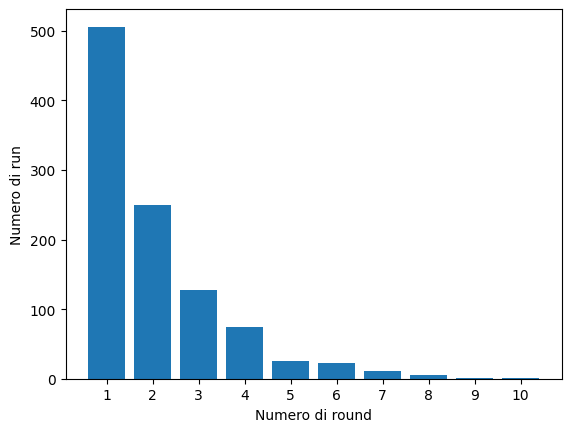
\includegraphics[width=\textwidth]{Grafico.png}
Il grafico suggerisce che la maggior parte delle $2^{10}$ esecuzioni dell'accordo bizantino viene completata nel primo round, con un dimezzamento del successo ad ogni round successivo.\\
Se in un qualche round per un processo affidabile $j$ risulta che $tally(j)\geq T$ e l'esito del lancio della moneta coincide con $maj(j)$, il round successivo l'accordo è certamente raggiunto perchè \textbf{BOH}
\end{document}